\section{Conception}
    Dans le but de limiter l'utilisation de la mémoire et de réduire le temps d'entraînement, les réseaux de neurones n'utilisent pas les images Full HD (1920x1080) à l'entrée, mais plutôt des images redimensionnées par un facteur de 4. Les images d'entrée des réseaux de neurones ont une résolution de 480x270. La sortie de tous les réseaux de neurones correspond à une matrice d'erreur de 16x9 éléments parce que les images sont divisées en 144 régions comme décrit à la section \ref{sec:definition_projet}. Les régions ont une résolution 30x30 pour les images d'entrée des réseaux de neurones (120x120 pour les images Full HD). Pour l'ensemble des réseaux de neurones développés, le champ récepteur des neurones de sortie est de 60x60 (240x240 pour les images Full HD) parce que nous avons émis l'hypothèse que le voisinage de chaque région a une influence sur la région correspondant au neurone de sortie. Chaque élément de la matrice d'erreur de 16x9 correspond à l'erreur quadratique de reconstruction de la région de l'image d'entrée correspondante. 

\subsection{Choix des métriques}
    L'entraînement se fait de façon non supervisée, donc il  a été décidé d'utiliser la fonction de coût d'entraînement du réseau définie par l'équation suivante. À l'aide de celle-ci, les réseaux de neurones apprennent à reconstruire les régions des images d'entraînement.
    
    \begin{equation}
        L = \sum_{i,j} \mathbf{S}_{i,j} \text{, où } \mathbf{S} \text{ est la matrice de sortie du réseau de neurone}
    \end{equation}
    
    Pour mesurer les performances des réseaux de neurones sur les données de validation et de test, l'utilisation des courbes ROC a été choisi puisque notre problème équivaut à un problème de classification deux classes où la classe est déterminée à l'aide d'un seuil. La courbe ROC est une bonne métrique dans ce cas. Pour permettre la comparaison des réseaux de neurones avec différents hyperparamètres et établir le meilleur type de réseau de neurones pour la situation, l'aire sous la courbe ROC a été utilisée. Plus l'aire sous la courbe est grande, plus que le réseau est bon. Pour calculer la courbe ROC, le nombre de vrais positifs et de faux positifs a été calculé pour différentes valeurs de seuil.

\subsection{Architecture des modèles}

    \begin{figure}[H]
        \centering
        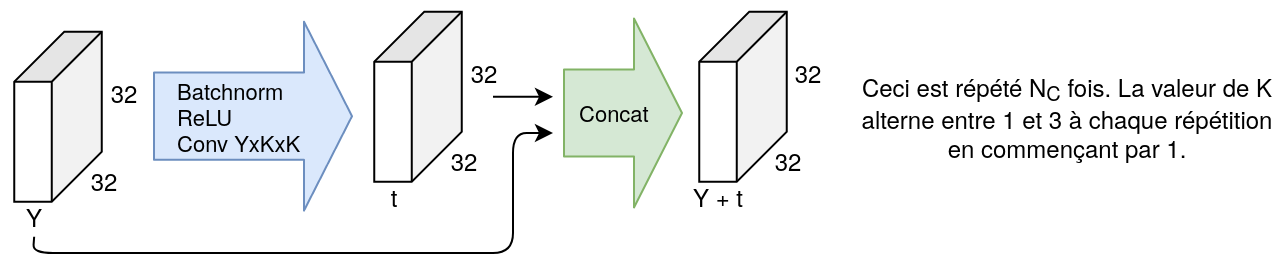
\includegraphics[width=12cm]{images/Architecture_DenseBlock.png}
        \caption{Architecture d'un bloc dense}
        \label{fig:architecture_bloc_dense}
    \end{figure}

    \begin{figure}[H]
        \centering
        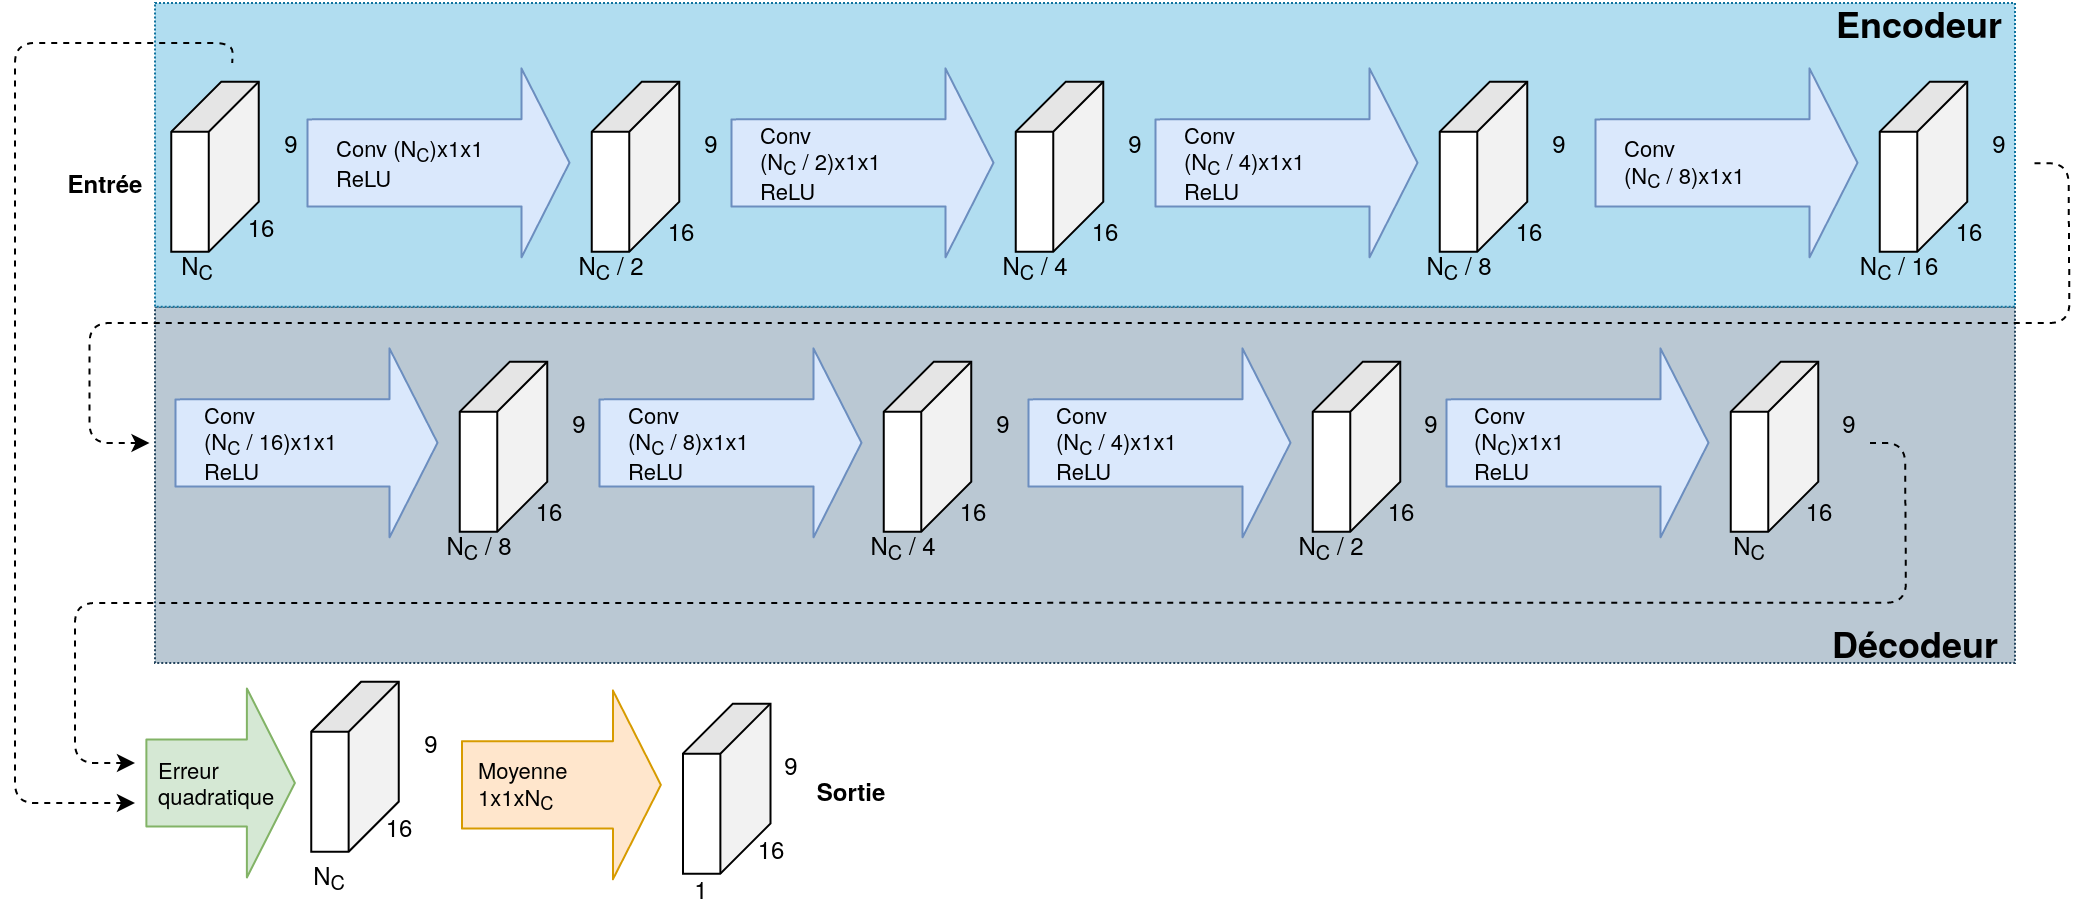
\includegraphics[width=17cm]{images/Architecture_FeatureAutoencoder.png}
        \caption{Architecture de l'auto-encodeur des caractéristiques}
        \label{fig:architecture_autoencoder_caracteristique}
    \end{figure}

\subsubsection{Auto-encodeur à base de couche convolutive appliqué sur l'image}
    \begin{figure}[H]
        \centering
        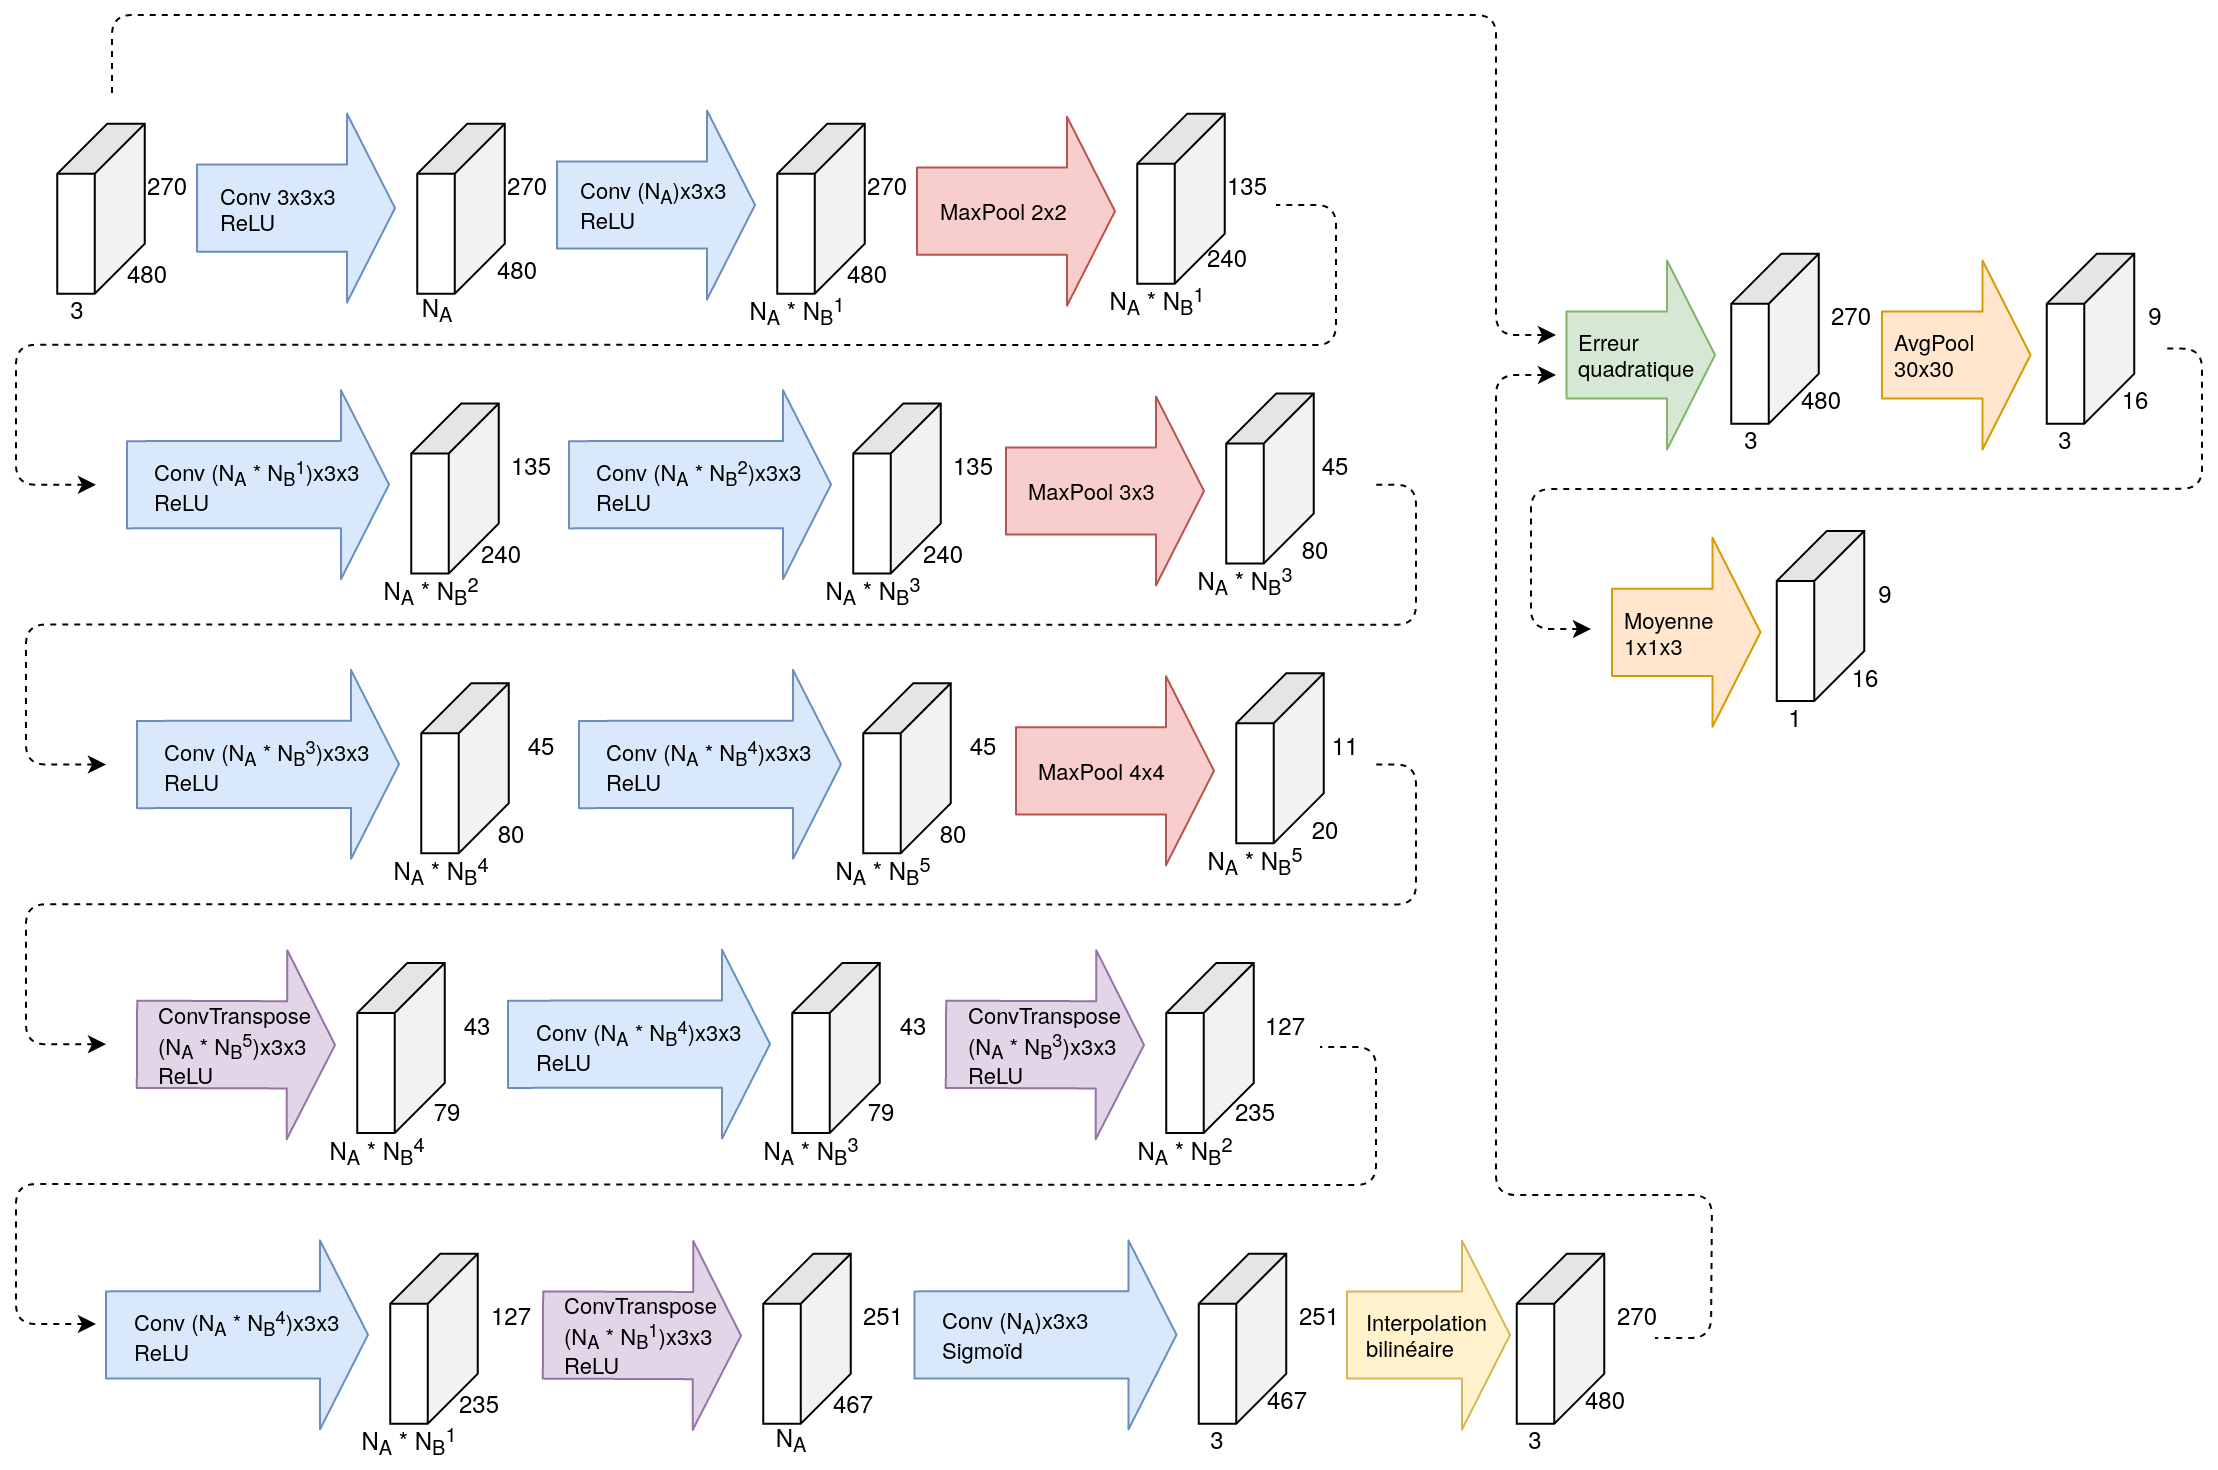
\includegraphics[width=17cm]{images/Architecture_CnnAutoencoder.png}
        \caption{Architecture de l'auto-encodeur à base de couche convolutive appliqué sur l'image}
        \label{fig:architecture_cnn_autoencoder}
    \end{figure}

\subsubsection{Auto-encodeur variationnel à base de couche convolutive appliqué sur l'image}
    \begin{figure}[H]
        \centering
        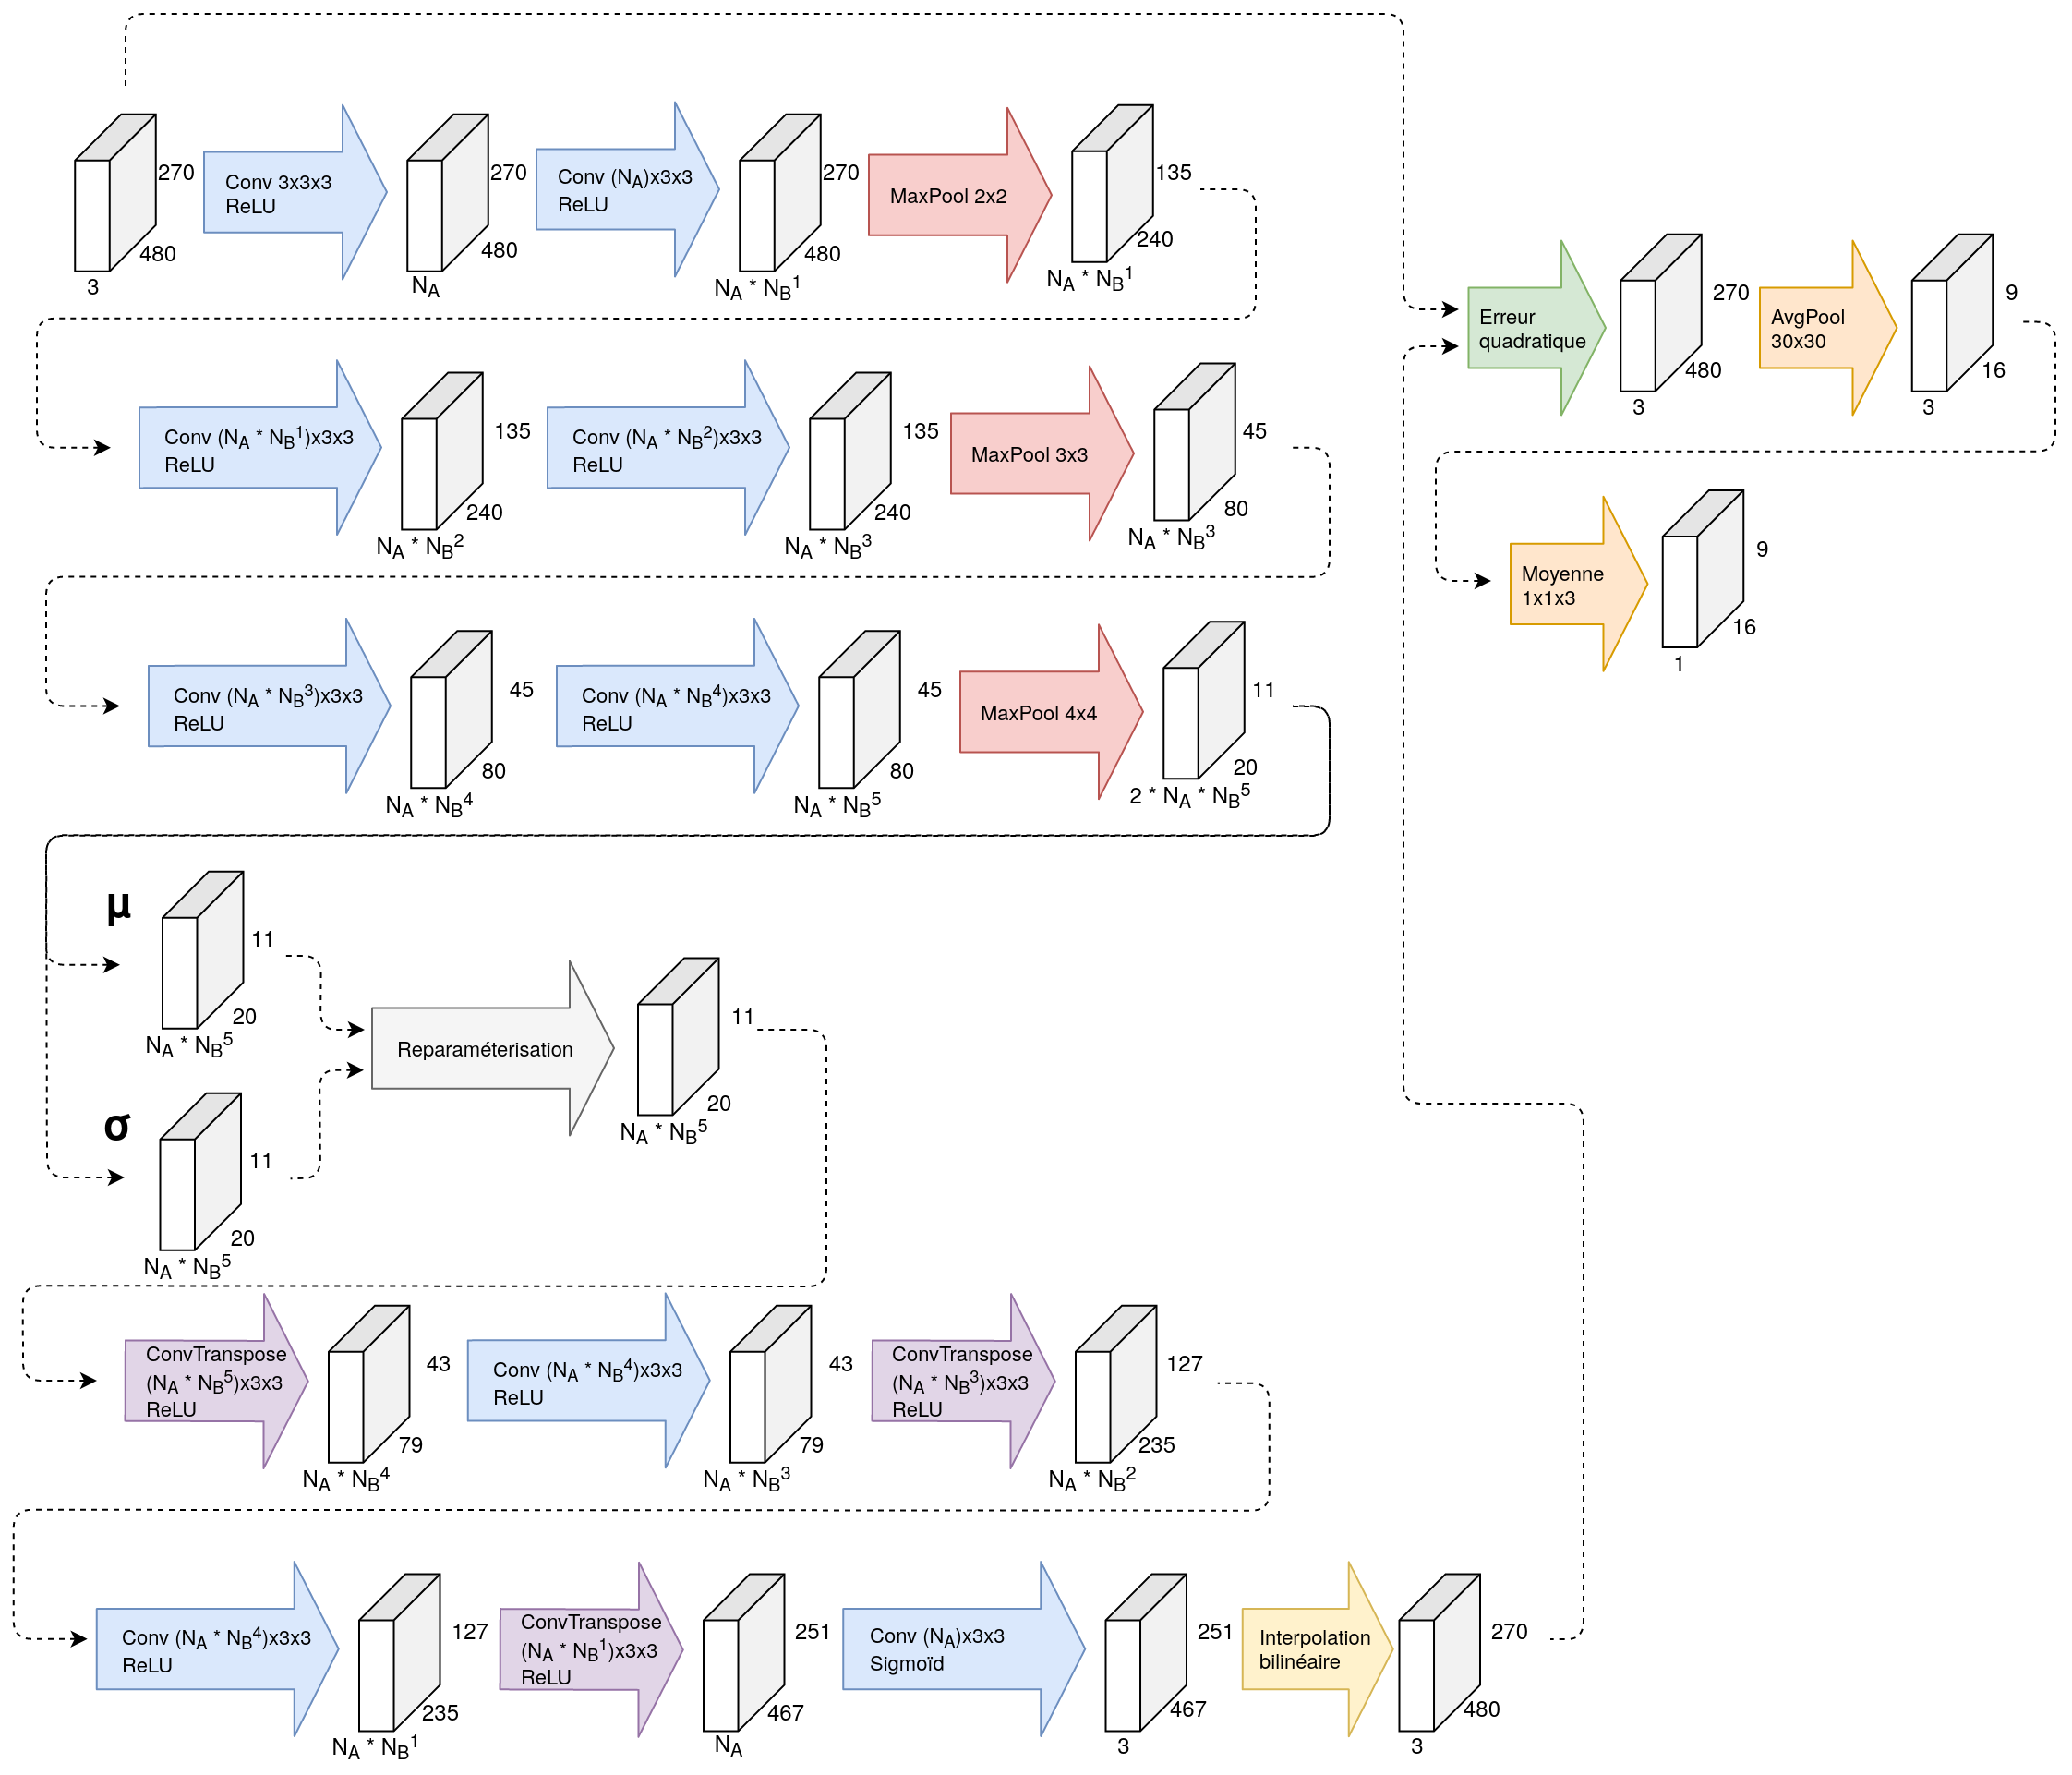
\includegraphics[width=17cm]{images/Architecture_CnnVae.png}
        \caption{Architecture de l'auto-encodeur variationnel à base de couche convolutive appliqué sur l'image}
        \label{fig:architecture_cnn_vae}
    \end{figure}

\subsubsection{Réseau de neurones convolutif extrayant des caractéristiques}
    \begin{figure}[H]
        \centering
        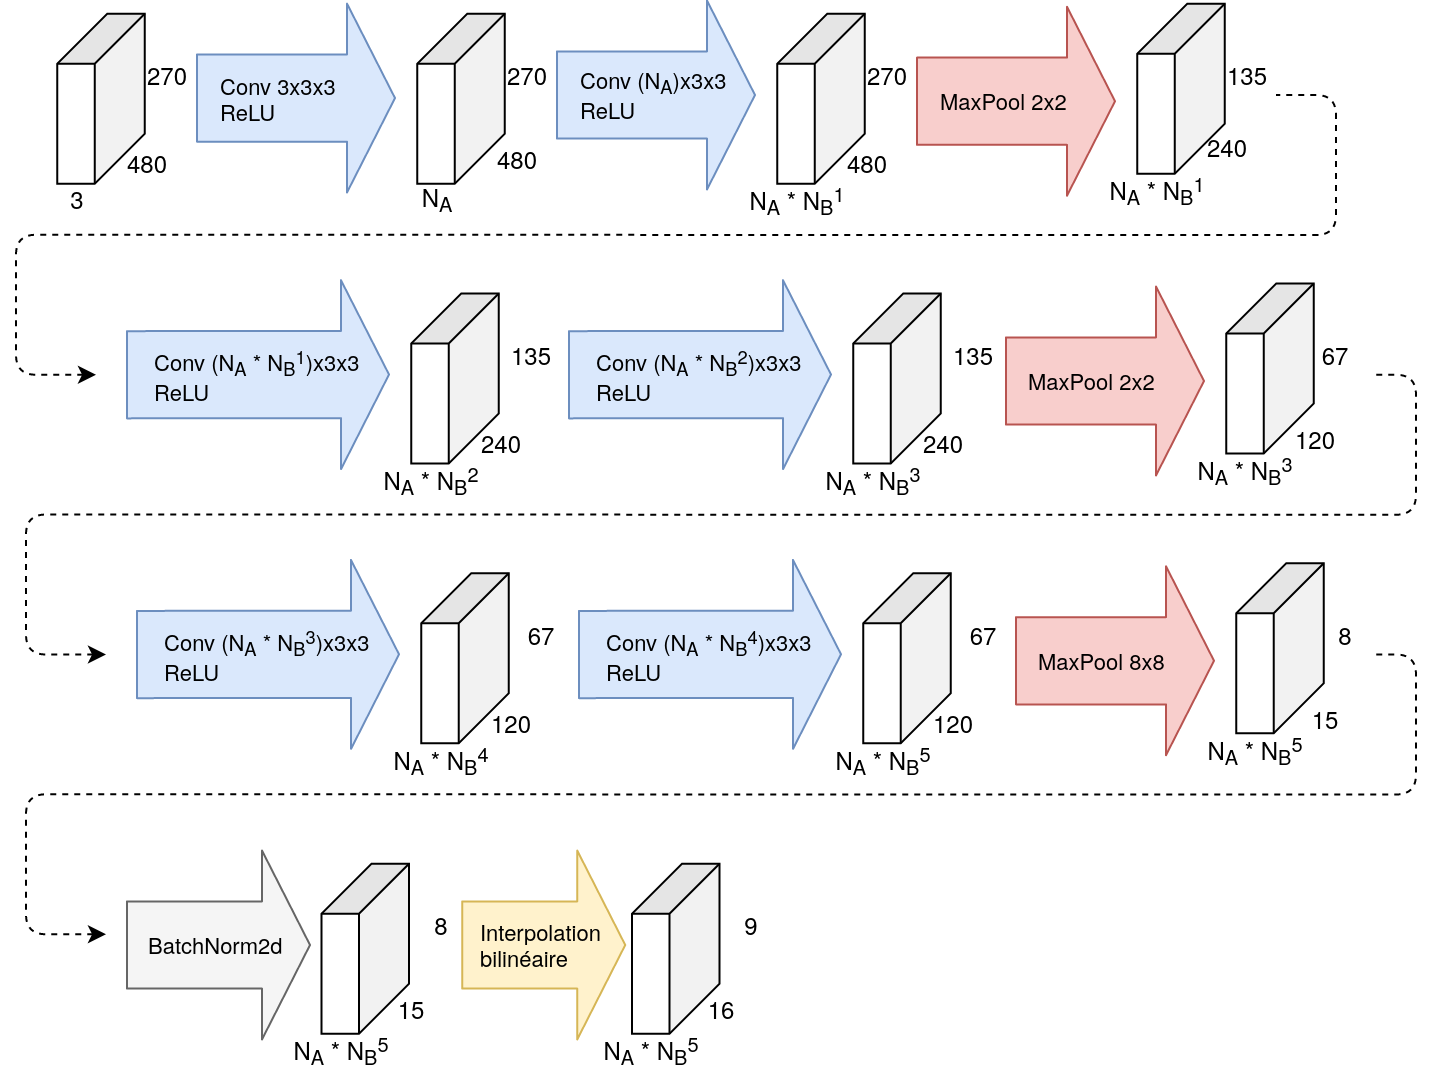
\includegraphics[width=17cm]{images/Architecture_SmallCnnWithAutoencoder.png}
        \caption{Architecture du réseau de neurones convolutif extrayant des caractéristiques}
        \label{fig:architecture_small_cnn}
    \end{figure}

\subsubsection{Réseau de neurones à base de blocs denses extrayant des caractéristiques}
    \begin{figure}[H]
        \centering
        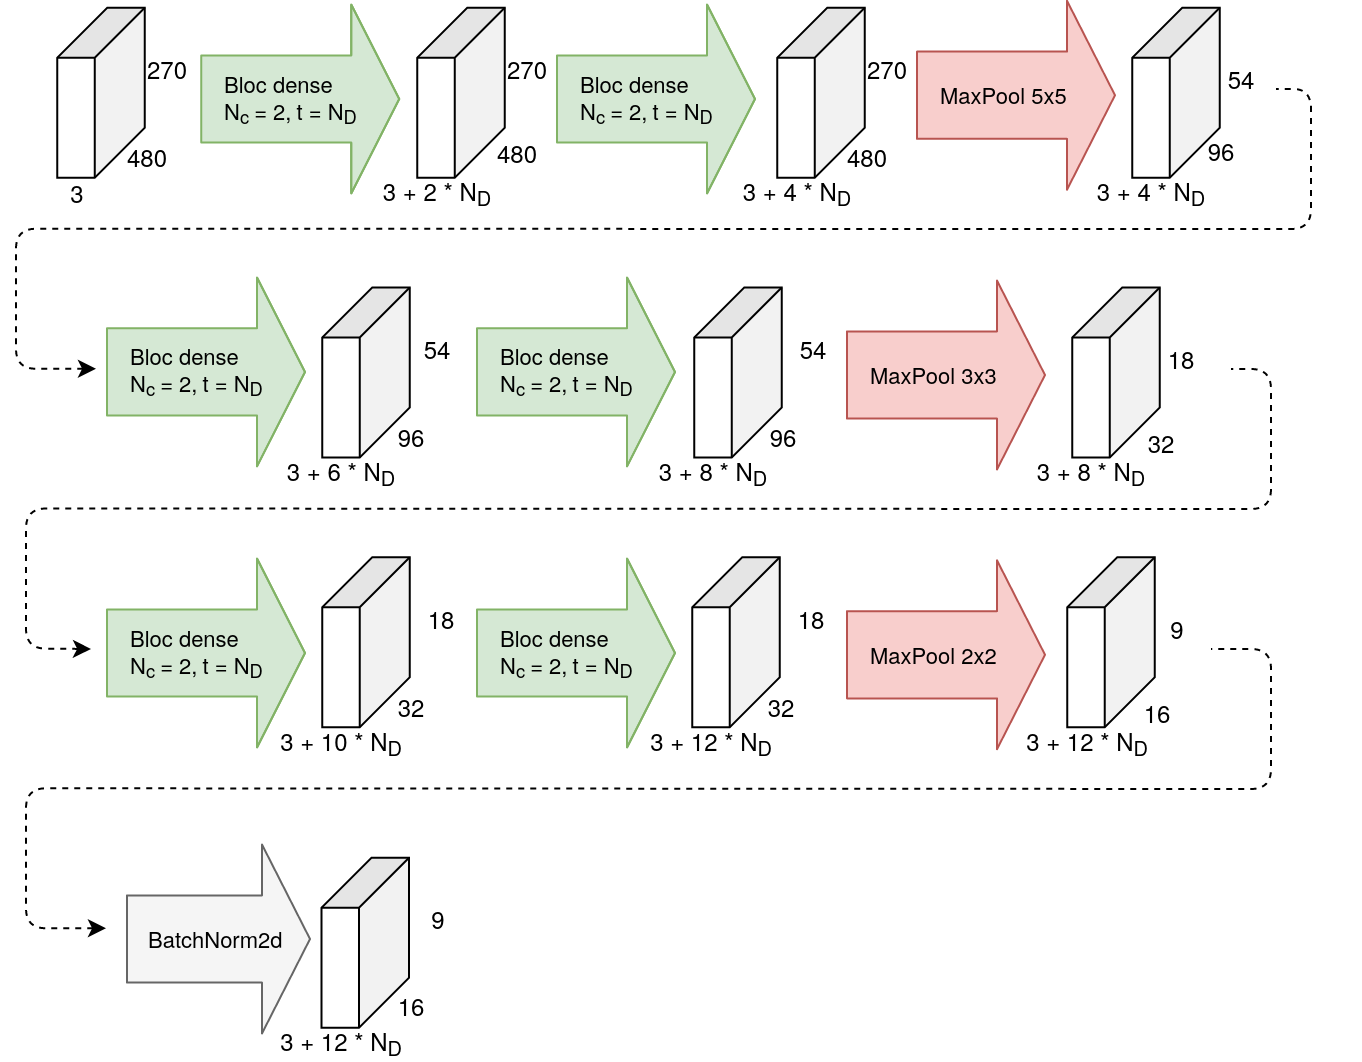
\includegraphics[width=17cm]{images/Architecture_SmallCnnWithAutoencoderDenseBlocks.png}
        \caption{Architecture du réseau de neurones à base de blocs denses extrayant des caractéristiques}
        \label{fig:architecture_small_cnn_dense_bloc}
    \end{figure}

\subsection{Réseau de neurones utilisant un \textit{backend} VGG16 pour l'extraction des caractéristiques}
    \begin{figure}[H]
        \centering
        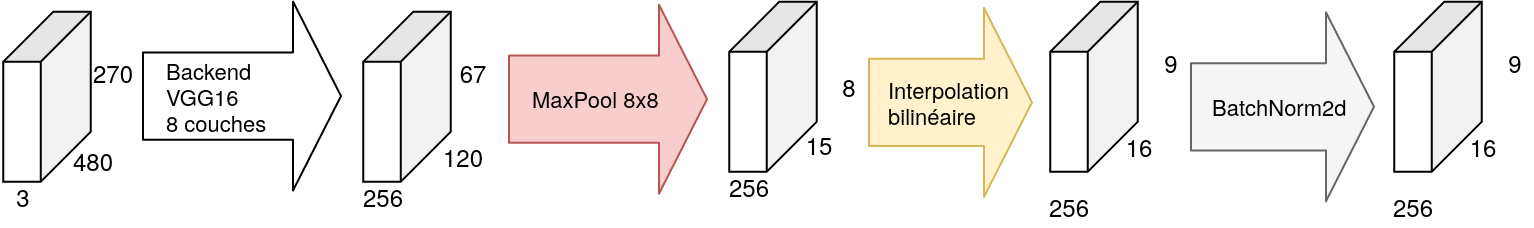
\includegraphics[width=12cm]{images/Architecture_Vgg16BackendAutoencoder.png}
        \caption{Architecture du réseau de neurones utilisant un \textit{backend} VGG16 pour l'extraction des caractéristiques}
        \label{fig:architecture_vgg16}
    \end{figure}

\subsection{Augmentation des données}
    